\documentclass{standalone}
\usepackage{tikz}
\usetikzlibrary{patterns, positioning}


\begin{document}
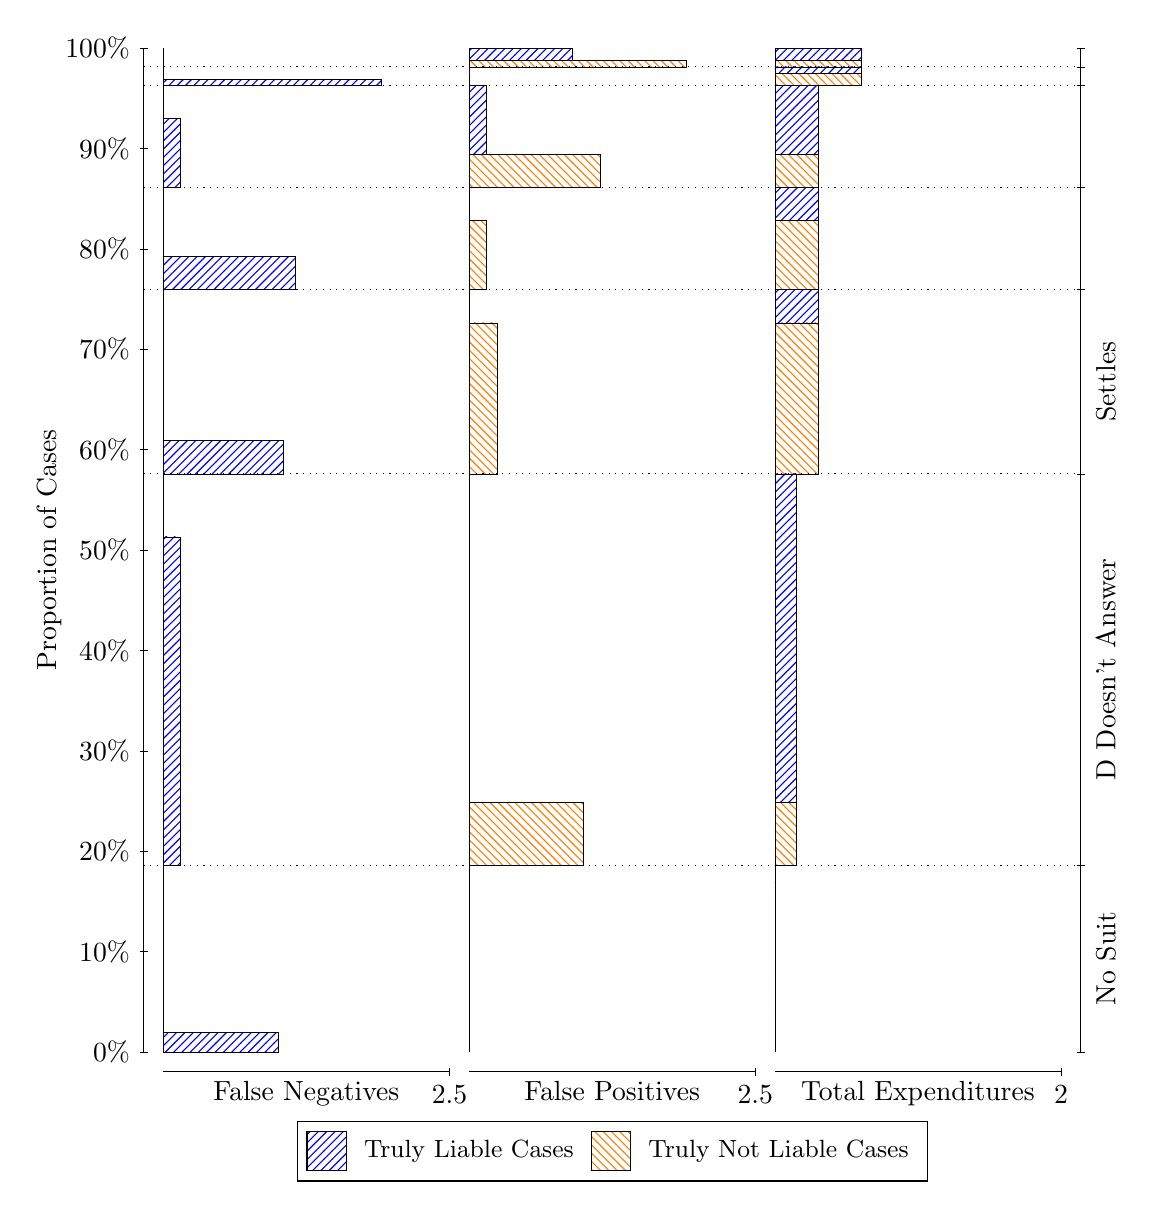
\begin{tikzpicture}
\draw[black, very thin] (1.5,1.75) -- (1.5,14.5);
\node[rotate=90, text=black, anchor=center] at (0.3, 8.125) {Proportion of Cases};
\draw[black, very thin] (1.45,1.75) -- (1.55,1.75);
\node[text=black, anchor=east] at (1.45, 1.75) {0\%};
\draw[black, very thin] (1.45,3.025) -- (1.55,3.025);
\node[text=black, anchor=east] at (1.45, 3.025) {10\%};
\draw[black, very thin] (1.45,4.3) -- (1.55,4.3);
\node[text=black, anchor=east] at (1.45, 4.3) {20\%};
\draw[black, very thin] (1.45,5.575) -- (1.55,5.575);
\node[text=black, anchor=east] at (1.45, 5.575) {30\%};
\draw[black, very thin] (1.45,6.85) -- (1.55,6.85);
\node[text=black, anchor=east] at (1.45, 6.85) {40\%};
\draw[black, very thin] (1.45,8.125) -- (1.55,8.125);
\node[text=black, anchor=east] at (1.45, 8.125) {50\%};
\draw[black, very thin] (1.45,9.4) -- (1.55,9.4);
\node[text=black, anchor=east] at (1.45, 9.4) {60\%};
\draw[black, very thin] (1.45,10.675) -- (1.55,10.675);
\node[text=black, anchor=east] at (1.45, 10.675) {70\%};
\draw[black, very thin] (1.45,11.95) -- (1.55,11.95);
\node[text=black, anchor=east] at (1.45, 11.95) {80\%};
\draw[black, very thin] (1.45,13.225) -- (1.55,13.225);
\node[text=black, anchor=east] at (1.45, 13.225) {90\%};
\draw[black, very thin] (1.45,14.5) -- (1.55,14.5);
\node[text=black, anchor=east] at (1.45, 14.5) {100\%};

\draw[black, very thin] (13.4,1.75) -- (13.4,14.5);
\draw[black, very thin] (13.35,1.75) -- (13.45,1.75);
\node[anchor=west] at (13.35, 1.75) {};
\draw[black, very thin] (13.35,4.1224) -- (13.45,4.1224);
\node[anchor=west] at (13.35, 4.1224) {};
\draw[black, very thin] (13.35,9.0921) -- (13.45,9.0921);
\node[anchor=west] at (13.35, 9.0921) {};
\draw[black, very thin] (13.35,11.432) -- (13.45,11.432);
\node[anchor=west] at (13.35, 11.432) {};
\draw[black, very thin] (13.35,12.727) -- (13.45,12.727);
\node[anchor=west] at (13.35, 12.727) {};
\draw[black, very thin] (13.35,14.022) -- (13.45,14.022);
\node[anchor=west] at (13.35, 14.022) {};
\draw[black, very thin] (13.35,14.261) -- (13.45,14.261);
\node[anchor=west] at (13.35, 14.261) {};
\draw[black, very thin] (13.35,14.5) -- (13.45,14.5);
\node[anchor=west] at (13.35, 14.5) {};

\draw[black, very thin, pattern color=blue, pattern=north east lines] (1.75,1.75) rectangle (3.2033,1.9996);
\draw[black, very thin, pattern color=orange, pattern=north west lines] (1.75,1.9996) rectangle (1.75,4.1224);
\draw[black, very thin, pattern color=blue, pattern=north east lines] (1.75,4.1224) rectangle (1.968,8.2905);
\draw[black, very thin, pattern color=orange, pattern=north west lines] (1.75,8.2905) rectangle (1.75,9.0921);
\draw[black, very thin, pattern color=blue, pattern=north east lines] (1.75,9.0921) rectangle (3.276,9.5154);
\draw[black, very thin, pattern color=orange, pattern=north west lines] (1.75,9.5154) rectangle (1.75,11.432);
\draw[black, very thin, pattern color=blue, pattern=north east lines] (1.75,11.432) rectangle (3.4213,11.851);
\draw[black, very thin, pattern color=orange, pattern=north west lines] (1.75,11.851) rectangle (1.75,12.727);
\draw[black, very thin, pattern color=blue, pattern=north east lines] (1.75,12.727) rectangle (1.968,13.602);
\draw[black, very thin, pattern color=orange, pattern=north west lines] (1.75,13.602) rectangle (1.75,14.022);
\draw[black, very thin, pattern color=blue, pattern=north east lines] (1.75,14.022) rectangle (4.5113,14.106);
\draw[black, very thin, pattern color=orange, pattern=north west lines] (1.75,14.106) rectangle (1.75,14.261);
\draw[black, very thin, pattern color=orange, pattern=north west lines] (1.75,14.261) rectangle (1.75,14.345);
\draw[black, very thin, pattern color=blue, pattern=north east lines] (1.75,14.345) rectangle (1.75,14.5);
\draw[black, very thin, pattern color=orange, pattern=north west lines] (5.6333,1.75) rectangle (5.6333,3.8728);
\draw[black, very thin, pattern color=blue, pattern=north east lines] (5.6333,3.8728) rectangle (5.6333,4.1224);
\draw[black, very thin, pattern color=orange, pattern=north west lines] (5.6333,4.1224) rectangle (7.0867,4.924);
\draw[black, very thin, pattern color=blue, pattern=north east lines] (5.6333,4.924) rectangle (5.6333,9.0921);
\draw[black, very thin, pattern color=orange, pattern=north west lines] (5.6333,9.0921) rectangle (5.9967,11.009);
\draw[black, very thin, pattern color=blue, pattern=north east lines] (5.6333,11.009) rectangle (5.6333,11.432);
\draw[black, very thin, pattern color=orange, pattern=north west lines] (5.6333,11.432) rectangle (5.8513,12.308);
\draw[black, very thin, pattern color=blue, pattern=north east lines] (5.6333,12.308) rectangle (5.6333,12.727);
\draw[black, very thin, pattern color=orange, pattern=north west lines] (5.6333,12.727) rectangle (7.3047,13.146);
\draw[black, very thin, pattern color=blue, pattern=north east lines] (5.6333,13.146) rectangle (5.8513,14.022);
\draw[black, very thin, pattern color=orange, pattern=north west lines] (5.6333,14.022) rectangle (5.6333,14.176);
\draw[black, very thin, pattern color=blue, pattern=north east lines] (5.6333,14.176) rectangle (5.6333,14.261);
\draw[black, very thin, pattern color=orange, pattern=north west lines] (5.6333,14.261) rectangle (8.3947,14.345);
\draw[black, very thin, pattern color=blue, pattern=north east lines] (5.6333,14.345) rectangle (6.9413,14.5);
\draw[black, very thin, pattern color=orange, pattern=north west lines] (9.5167,1.75) rectangle (9.5167,3.8728);
\draw[black, very thin, pattern color=blue, pattern=north east lines] (9.5167,3.8728) rectangle (9.5167,4.1224);
\draw[black, very thin, pattern color=orange, pattern=north west lines] (9.5167,4.1224) rectangle (9.7892,4.924);
\draw[black, very thin, pattern color=blue, pattern=north east lines] (9.5167,4.924) rectangle (9.7892,9.0921);
\draw[black, very thin, pattern color=orange, pattern=north west lines] (9.5167,9.0921) rectangle (10.062,11.009);
\draw[black, very thin, pattern color=blue, pattern=north east lines] (9.5167,11.009) rectangle (10.062,11.432);
\draw[black, very thin, pattern color=orange, pattern=north west lines] (9.5167,11.432) rectangle (10.062,12.308);
\draw[black, very thin, pattern color=blue, pattern=north east lines] (9.5167,12.308) rectangle (10.062,12.727);
\draw[black, very thin, pattern color=orange, pattern=north west lines] (9.5167,12.727) rectangle (10.062,13.146);
\draw[black, very thin, pattern color=blue, pattern=north east lines] (9.5167,13.146) rectangle (10.062,14.022);
\draw[black, very thin, pattern color=orange, pattern=north west lines] (9.5167,14.022) rectangle (10.607,14.176);
\draw[black, very thin, pattern color=blue, pattern=north east lines] (9.5167,14.176) rectangle (10.607,14.261);
\draw[black, very thin, pattern color=orange, pattern=north west lines] (9.5167,14.261) rectangle (10.607,14.345);
\draw[black, very thin, pattern color=blue, pattern=north east lines] (9.5167,14.345) rectangle (10.607,14.5);
\draw[black, dotted] (1.5,4.1224) -- (13.4,4.1224);
\draw[black, dotted] (1.5,9.0921) -- (13.4,9.0921);
\draw[black, dotted] (1.5,11.432) -- (13.4,11.432);
\draw[black, dotted] (1.5,12.727) -- (13.4,12.727);
\draw[black, dotted] (1.5,14.022) -- (13.4,14.022);
\draw[black, dotted] (1.5,14.261) -- (13.4,14.261);
\draw[black, very thin] (1.75,1.5) -- (5.3833,1.5);
\node[text=black, anchor=north] at (3.5667, 1.5) {False Negatives};
\draw[black, very thin] (5.3833,1.45) -- (5.3833,1.55);
\node[text=black, anchor=north] at (5.3833, 1.45) {2.5};

\draw[black, very thin] (5.6333,1.5) -- (9.2667,1.5);
\node[text=black, anchor=north] at (7.45, 1.5) {False Positives};
\draw[black, very thin] (9.2667,1.45) -- (9.2667,1.55);
\node[text=black, anchor=north] at (9.2667, 1.45) {2.5};

\draw[black, very thin] (9.5167,1.5) -- (13.15,1.5);
\node[text=black, anchor=north] at (11.333, 1.5) {Total Expenditures};
\draw[black, very thin] (13.15,1.45) -- (13.15,1.55);
\node[text=black, anchor=north] at (13.15, 1.45) {2};

\node[text=black, centered, rotate=90] at (13.72, 2.9362) {No Suit};
\node[text=black, centered, rotate=90] at (13.72, 6.6072) {D Doesn't Answer};
\node[text=black, centered, rotate=90] at (13.72, 10.262) {Settles};





\draw (7.449999999999999,1.5) node[draw=none] (baseCoordinate) {};
\begin{scope}[align=center]
        \matrix[scale=0.5, draw=black, below=0.5cm of baseCoordinate, nodes={draw}, column sep=0.1cm]{
            \node[rectangle, draw, minimum width=0.5cm, minimum height=0.5cm, pattern color=blue, pattern=north east lines] {}; &
            \node[draw=none, font=\small, text=black] (B) {Truly Liable Cases}; &
            \node[rectangle, draw, minimum width=0.5cm, minimum height=0.5cm, pattern color=orange, pattern=north west lines] {}; &
            \node[draw=none, font=\small, text=black] (B) {Truly Not Liable Cases}; \\
            };
\end{scope}

\end{tikzpicture}
\end{document}